\documentclass[conference]{IEEEtran}

\usepackage{amsmath}
\usepackage{graphicx}
\usepackage{booktabs}
\usepackage{url}

\title{Evaluating the Impact of Robot Carrying Capacity on
Deadline-Constrained Warehouse Planning}

\author{
\IEEEauthorblockN{Paolo Nicolini}
\IEEEauthorblockA{
University of Genoa\\
Research Track II
}
}

\begin{document}

\maketitle

\begin{abstract}
Robot carrying capacity can influence both the physical execution of warehouse
tasks and the computational difficulty of planning them. This work evaluates
the effect of increasing a warehouse robot's carrying capacity from one to two
packages in a deadline-constrained PDDL+ planning domain. The original
single-package model was generalized using numeric fluents for current load
and maximum capacity. A controlled factorial experiment varied package count,
deadline tightness, and package distribution while evaluating both capacity
configurations on identical warehouse scenarios. Twenty reproducible seeds
were generated for each condition, producing 160 paired scenarios and 320
ENHSP planner executions. Capacity one solved 72.50\% of the scenarios,
compared with 93.75\% for capacity two. An exact McNemar test showed a
significant paired difference ($p=1.16\times10^{-10}$). Among the 116
scenarios solved by both capacities, capacity two reduced mean makespan by
28.54\%, plan length by 23.34\%, expanded nodes by 61.93\%, and evaluated
states by 57.80\%. The results also show that the benefit of additional
capacity depends strongly on package layout.
\end{abstract}

\begin{IEEEkeywords}
automated planning, PDDL+, warehouse robotics, numeric planning,
carrying capacity, ENHSP
\end{IEEEkeywords}

\section{Introduction}

Robotized warehouse systems introduce planning problems involving routing,
order handling, task allocation, and autonomous vehicle operation
\cite{azadeh2019,barros2021}. Large-scale robotic fulfillment systems have
also demonstrated the practical need to coordinate fleets of autonomous
vehicles in warehouse environments \cite{wurman2008}, while broader
warehousing research highlights increasingly time-critical and automated
fulfillment operations \cite{boysen2019}. One robot characteristic that can
directly affect these operations is carrying capacity.

A robot restricted to one package may need to revisit the same warehouse area
several times, whereas a robot with greater capacity may collect multiple
packages during a single visit. However, the benefit is not necessarily
universal. If packages are spatially separated, additional capacity may not
reduce travel. Under tight delivery deadlines, capacity may also determine
whether a feasible plan exists.

Warehouse transportation tasks are related to classical pickup-and-delivery
problems, where routing decisions interact with vehicle capacity, precedence,
and temporal constraints \cite{dumas1991,savelsbergh1995}. In this work, the
problem is instead studied from an automated-planning perspective using an
explicit symbolic and numeric model.

PDDL2.1 extended classical planning with durative actions and numeric fluents
for temporal planning \cite{fox2003}. PDDL+ subsequently introduced autonomous
processes and events, enabling the representation of mixed
discrete-continuous systems \cite{fox2006}. Planning such domains requires
search methods that reason about numeric evolution, processes, and event
timing \cite{coles2014,piotrowski2016}. Numeric heuristic-search techniques
further extend the range of expressive planning problems that can be addressed
\cite{scala2016subgoal,scala2016interval,scala2020}.

The research question addressed in this work is:

\emph{How does increasing robot carrying capacity from one to two packages
affect solvability, mission makespan, plan length, and planning complexity
under different package distributions and deadline constraints?}

The main contributions are:
\begin{itemize}
    \item a generalized capacity-aware PDDL+ warehouse model;
    \item a controlled paired experiment over 160 warehouse scenarios;
    \item automated ENHSP execution and metric extraction;
    \item statistical analysis of feasibility and planning efficiency;
    \item a ROS2 and Jupyter interface for interactive reproduction.
\end{itemize}

\section{Related Work}

\subsection{PDDL+ and Numeric Planning}

Fox and Long first extended PDDL with durative actions and numeric fluents in
PDDL2.1 \cite{fox2003}. PDDL+ subsequently added autonomous processes and
events, allowing deterministic mixed discrete-continuous domains to be modeled
explicitly \cite{fox2006}. This representation is suitable for warehouse tasks
in which robot motion and deadline countdowns evolve continuously while
pickups and deliveries remain discrete actions.

Coles and Coles studied planning with PDDL+ events and linear processes
\cite{coles2014}, while Piotrowski et al.\ investigated heuristic planning
methods for PDDL+ domains \cite{piotrowski2016}. These works illustrate the
additional search challenges introduced by autonomous numeric evolution and
event timing.

Scala, Haslum, and Thi\'ebaux extended heuristic subgoaling techniques to
numeric planning, including admissible heuristics for optimal numeric search
\cite{scala2016subgoal}. Interval-based relaxations were subsequently proposed
for more general numeric planning problems \cite{scala2016interval}, while
later work further developed subgoaling methods for satisficing and optimal
numeric planning \cite{scala2020}. Together, these methods provide the
planning background for the ENHSP-based experimental framework used here.

\subsection{Robotic Warehouses and Pickup-and-Delivery}

Azadeh et al.\ survey robotized and automated warehouse systems and identify
routing, order picking, assignment, and system control as major research
problems \cite{azadeh2019}. Barros and Nascimento provide a complementary
survey focused on robotic mobile fulfillment systems \cite{barros2021}.
Wurman et al.\ describe the coordination of large fleets of cooperative
autonomous vehicles in the Kiva warehouse system \cite{wurman2008},
demonstrating the practical relevance of large-scale robotic material
handling. Boysen et al.\ review warehousing in the e-commerce era and discuss
the growing importance of automation, rapid order fulfillment, and new
operational planning challenges \cite{boysen2019}.

The transportation component is closely related to pickup-and-delivery
routing. Dumas et al.\ study pickup-and-delivery with time windows, combining
routing, capacity, precedence, and temporal constraints \cite{dumas1991}.
Savelsbergh and Sol provide a broader formulation of the general
pickup-and-delivery problem \cite{savelsbergh1995}.

The present work differs by treating carrying capacity as an experimental
variable inside a PDDL+ planning model and evaluating its influence not only on
mission efficiency but also on planner solvability and search complexity.

\section{Methodology}

\subsection{Warehouse Model}

The PDDL+ domain contains robots, packages, and locations. The fixed warehouse
topology includes a dock, two aisles, and a shipping location.

Robot movement is represented using the actions \texttt{start-move} and
\texttt{end-move}, together with the continuous \texttt{robot-transit}
process. The remaining travel distance decreases continuously while the robot
is moving.

Each package has a numeric fluent
\texttt{time-remaining}. For undelivered packages, the autonomous
\texttt{package-aging} process decreases this value at unit rate:
\begin{equation}
\frac{d}{dt}\mathrm{timeRemaining}(p)=-1.
\end{equation}

When the remaining time reaches zero, a \texttt{deadline-breach} event marks
the package as late. Delivery is permitted only while the package deadline has
not been missed.

\subsection{Generalized Carrying Capacity}

The original model used the Boolean predicate \texttt{hand-empty}, enforcing a
maximum capacity of one package.

The generalized model replaces it with:
\begin{itemize}
    \item \texttt{current-load(robot)};
    \item \texttt{max-capacity(robot)}.
\end{itemize}

A pickup is permitted when
\begin{equation}
\mathrm{currentLoad}(r)<\mathrm{maxCapacity}(r).
\end{equation}

Pickup increments the current load by one, while intermediate drop and
successful delivery decrement it by one. The same domain can therefore
represent both capacity-one and capacity-two robots by changing only the
initial value of \texttt{max-capacity}.

This preserves the warehouse topology, package definitions, deadlines,
actions, and planner configuration across both experimental conditions.

\subsection{Package Handling and Planning Goal}

Three discrete actions control package manipulation:
\texttt{pick}, \texttt{drop-intermediate}, and
\texttt{deliver-package}. A pickup marks a package as carried and increments
the robot load. An intermediate drop places the package at the robot's current
location and decrements the load. A delivery is valid only when the robot is
carrying the package at its target location and the package deadline has not
been violated.

For a capacity-two robot, the pickup precondition can remain satisfied after
the first pickup. This allows two packages to be transported simultaneously
when their locations and route structure make this useful.

The goal of every generated problem is the successful delivery of all
packages. Consequently, the planner must jointly reason about movement,
package manipulation, carrying capacity, and the continuous countdown of
delivery deadlines.

\section{Experimental Setup}

Four factors are considered:
\begin{itemize}
    \item carrying capacity: 1 or 2;
    \item package count: 2 or 3;
    \item deadline mode: relaxed or tight;
    \item package layout: clustered or distributed.
\end{itemize}

In clustered scenarios, packages occupy the same aisle. In distributed
two-package scenarios, one package is located in each aisle. For three-package
distributed scenarios, two packages share one aisle and the remaining package
is placed in the other.

The deadline ranges used by the generator are shown in
Table~\ref{tab:deadlines}. Tight ranges intentionally produce scenarios in
which repeated travel can make timely delivery impossible.

\begin{table}[t]
\caption{Generated Deadline Ranges}
\centering
\begin{tabular}{ccc}
\toprule
Packages & Relaxed & Tight \\
\midrule
2 & 20--30 & 7--12 \\
3 & 25--40 & 11--16 \\
\bottomrule
\end{tabular}
\label{tab:deadlines}
\end{table}

The warehouse travel distances are fixed: dock--aisle A and aisle
A--shipping require 2 time units, while dock--aisle B and aisle B--shipping
require 3.

Twenty reproducible seeds are generated for each combination of package count,
deadline mode, and layout:
\begin{equation}
2\times2\times2\times20=160
\end{equation}
distinct scenarios. Each is solved under both capacity conditions, producing
320 planner executions.

The scenarios are paired: package positions, deadlines, warehouse geometry,
and all other initial conditions remain identical while only carrying capacity
changes.

Scenario generation is fully automated. Each instance is associated with a
scenario identifier, package count, layout mode, deadline mode, and
reproducible random seed. Separate pseudo-random generators are used for
layout and deadline generation. Therefore, changing the spatial layout does
not unintentionally alter the deadline values associated with the same seed
and package-count condition.

For every scenario, the generator creates two problem files that differ only
in the initial value of \texttt{max-capacity}. This paired construction is
important because performance differences can be attributed to carrying
capacity rather than to differences between problem instances.

All problems are solved with ENHSP using the \texttt{opt-hrmax}
configuration and a timeout of 120 seconds.

The collected metrics are:
\begin{itemize}
    \item solved/unsolvable status;
    \item plan length;
    \item mission makespan;
    \item expanded nodes;
    \item evaluated states;
    \item planning time.
\end{itemize}

Solvability is analyzed with an exact McNemar test. Quantitative metrics are
compared with the Wilcoxon signed-rank test using scenarios solved under both
capacities.

Three ENHSP runs reported invalid negative planning-time measurements. These
values were treated as missing. Two occurred among jointly solved scenarios,
leaving 114 valid runtime pairs.

\subsection{Experiment Automation and Reproducibility}

The experimental pipeline is implemented in Python. It generates the PDDL+
problem files, invokes ENHSP, enforces the timeout, stores complete raw planner
output, extracts the relevant metrics, and associates each run with its
scenario metadata. Processed results are written to CSV files for subsequent
statistical analysis.

The project also exposes the planner through a ROS2 node. Planning requests
are sent through the topic \texttt{/warehouse\_experiment/request}, while
results are published on \texttt{/warehouse\_experiment/result}. An
interactive Jupyter notebook acts as a client, allowing a user to select a
scenario and capacity and execute the same ENHSP pipeline used by the batch
experiment. The notebook additionally reproduces the principal analyses and
figures from the final dataset.

\section{Results}

\subsection{Solvability}

Capacity one solved 116 of 160 scenarios (72.50\%), while capacity two solved
150 (93.75\%), an increase of 21.25 percentage points.

\begin{table}[t]
\caption{Paired Solvability Outcomes}
\centering
\begin{tabular}{lcc}
\toprule
 & Cap. 2 solved & Cap. 2 unsolved \\
\midrule
Cap. 1 solved   & 116 & 0  \\
Cap. 1 unsolved & 34  & 10 \\
\bottomrule
\end{tabular}
\label{tab:solvability}
\end{table}

All 34 discordant pairs favored capacity two. The exact McNemar test produced
$p=1.16\times10^{-10}$.

Figure~\ref{fig:success} shows that the effect depends strongly on the
experimental condition.

\begin{figure}[t]
\centering
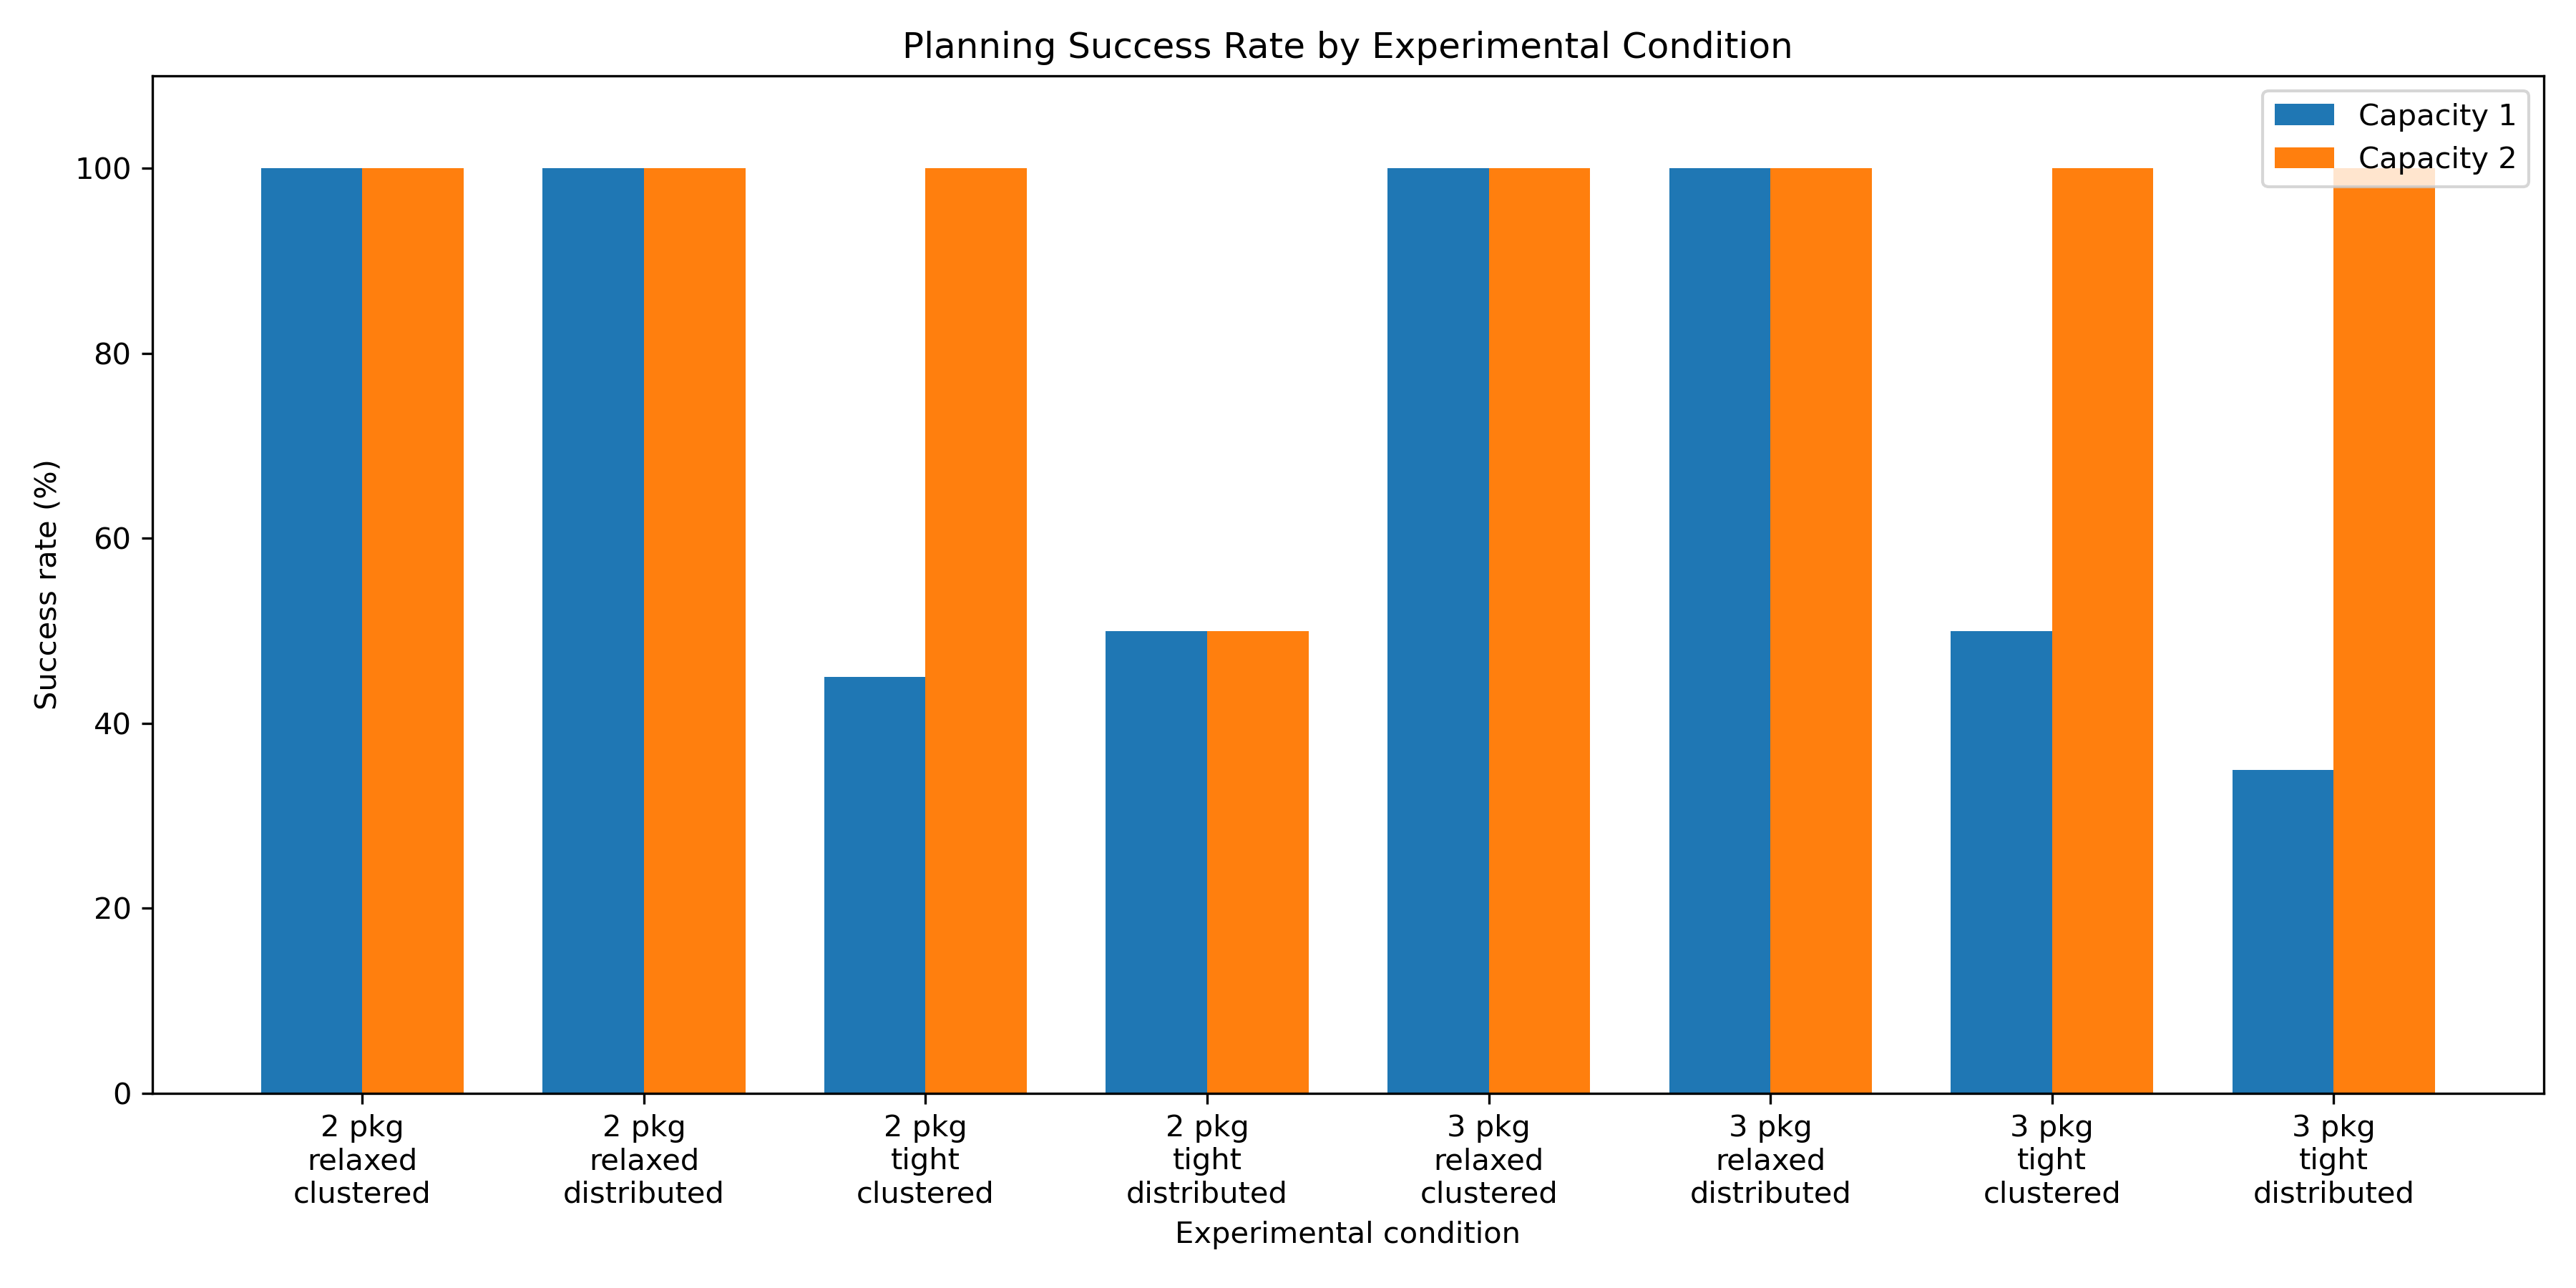
\includegraphics[width=\columnwidth]{figures/success_rate_by_condition.png}
\caption{Planning success rate by experimental condition.}
\label{fig:success}
\end{figure}

Under relaxed deadlines, both capacities solved every scenario. Under tight
deadlines, success changed from 45\% to 100\% for two clustered packages,
50\% to 100\% for three clustered packages, and 35\% to 100\% for three
distributed packages. For two tight distributed packages, both capacities
remained at 50\%.

Table~\ref{tab:condition_success} reports all condition-level success rates.

\begin{table}[t]
\caption{Success Rate by Experimental Condition}
\centering
\begin{tabular}{cccrr}
\toprule
Pkg. & Deadline & Layout & Cap. 1 & Cap. 2 \\
\midrule
2 & Relaxed & Clustered   & 100\% & 100\% \\
2 & Relaxed & Distributed & 100\% & 100\% \\
2 & Tight   & Clustered   & 45\%  & 100\% \\
2 & Tight   & Distributed & 50\%  & 50\%  \\
3 & Relaxed & Clustered   & 100\% & 100\% \\
3 & Relaxed & Distributed & 100\% & 100\% \\
3 & Tight   & Clustered   & 50\%  & 100\% \\
3 & Tight   & Distributed & 35\%  & 100\% \\
\bottomrule
\end{tabular}
\label{tab:condition_success}
\end{table}

The two-package tight distributed condition is especially informative. In this
case, increasing capacity alone cannot remove the need to visit both aisles,
and the observed feasibility rate is identical under both capacities.

\subsection{Mission Efficiency}

Among the 116 scenarios solved by both capacities, mean makespan decreased from
11.983 to 8.500 time units, corresponding to a 28.54\% mean paired reduction.
Capacity two produced lower makespan in 86 pairs and tied in 30; it was never
worse. The Wilcoxon test produced $p=4.89\times10^{-17}$.

Mean plan length decreased from 26.931 to 20.483 actions, a 23.34\% mean
paired reduction, with the same 86 improvements and 30 ties
($p=4.89\times10^{-17}$).

\begin{figure}[t]
\centering
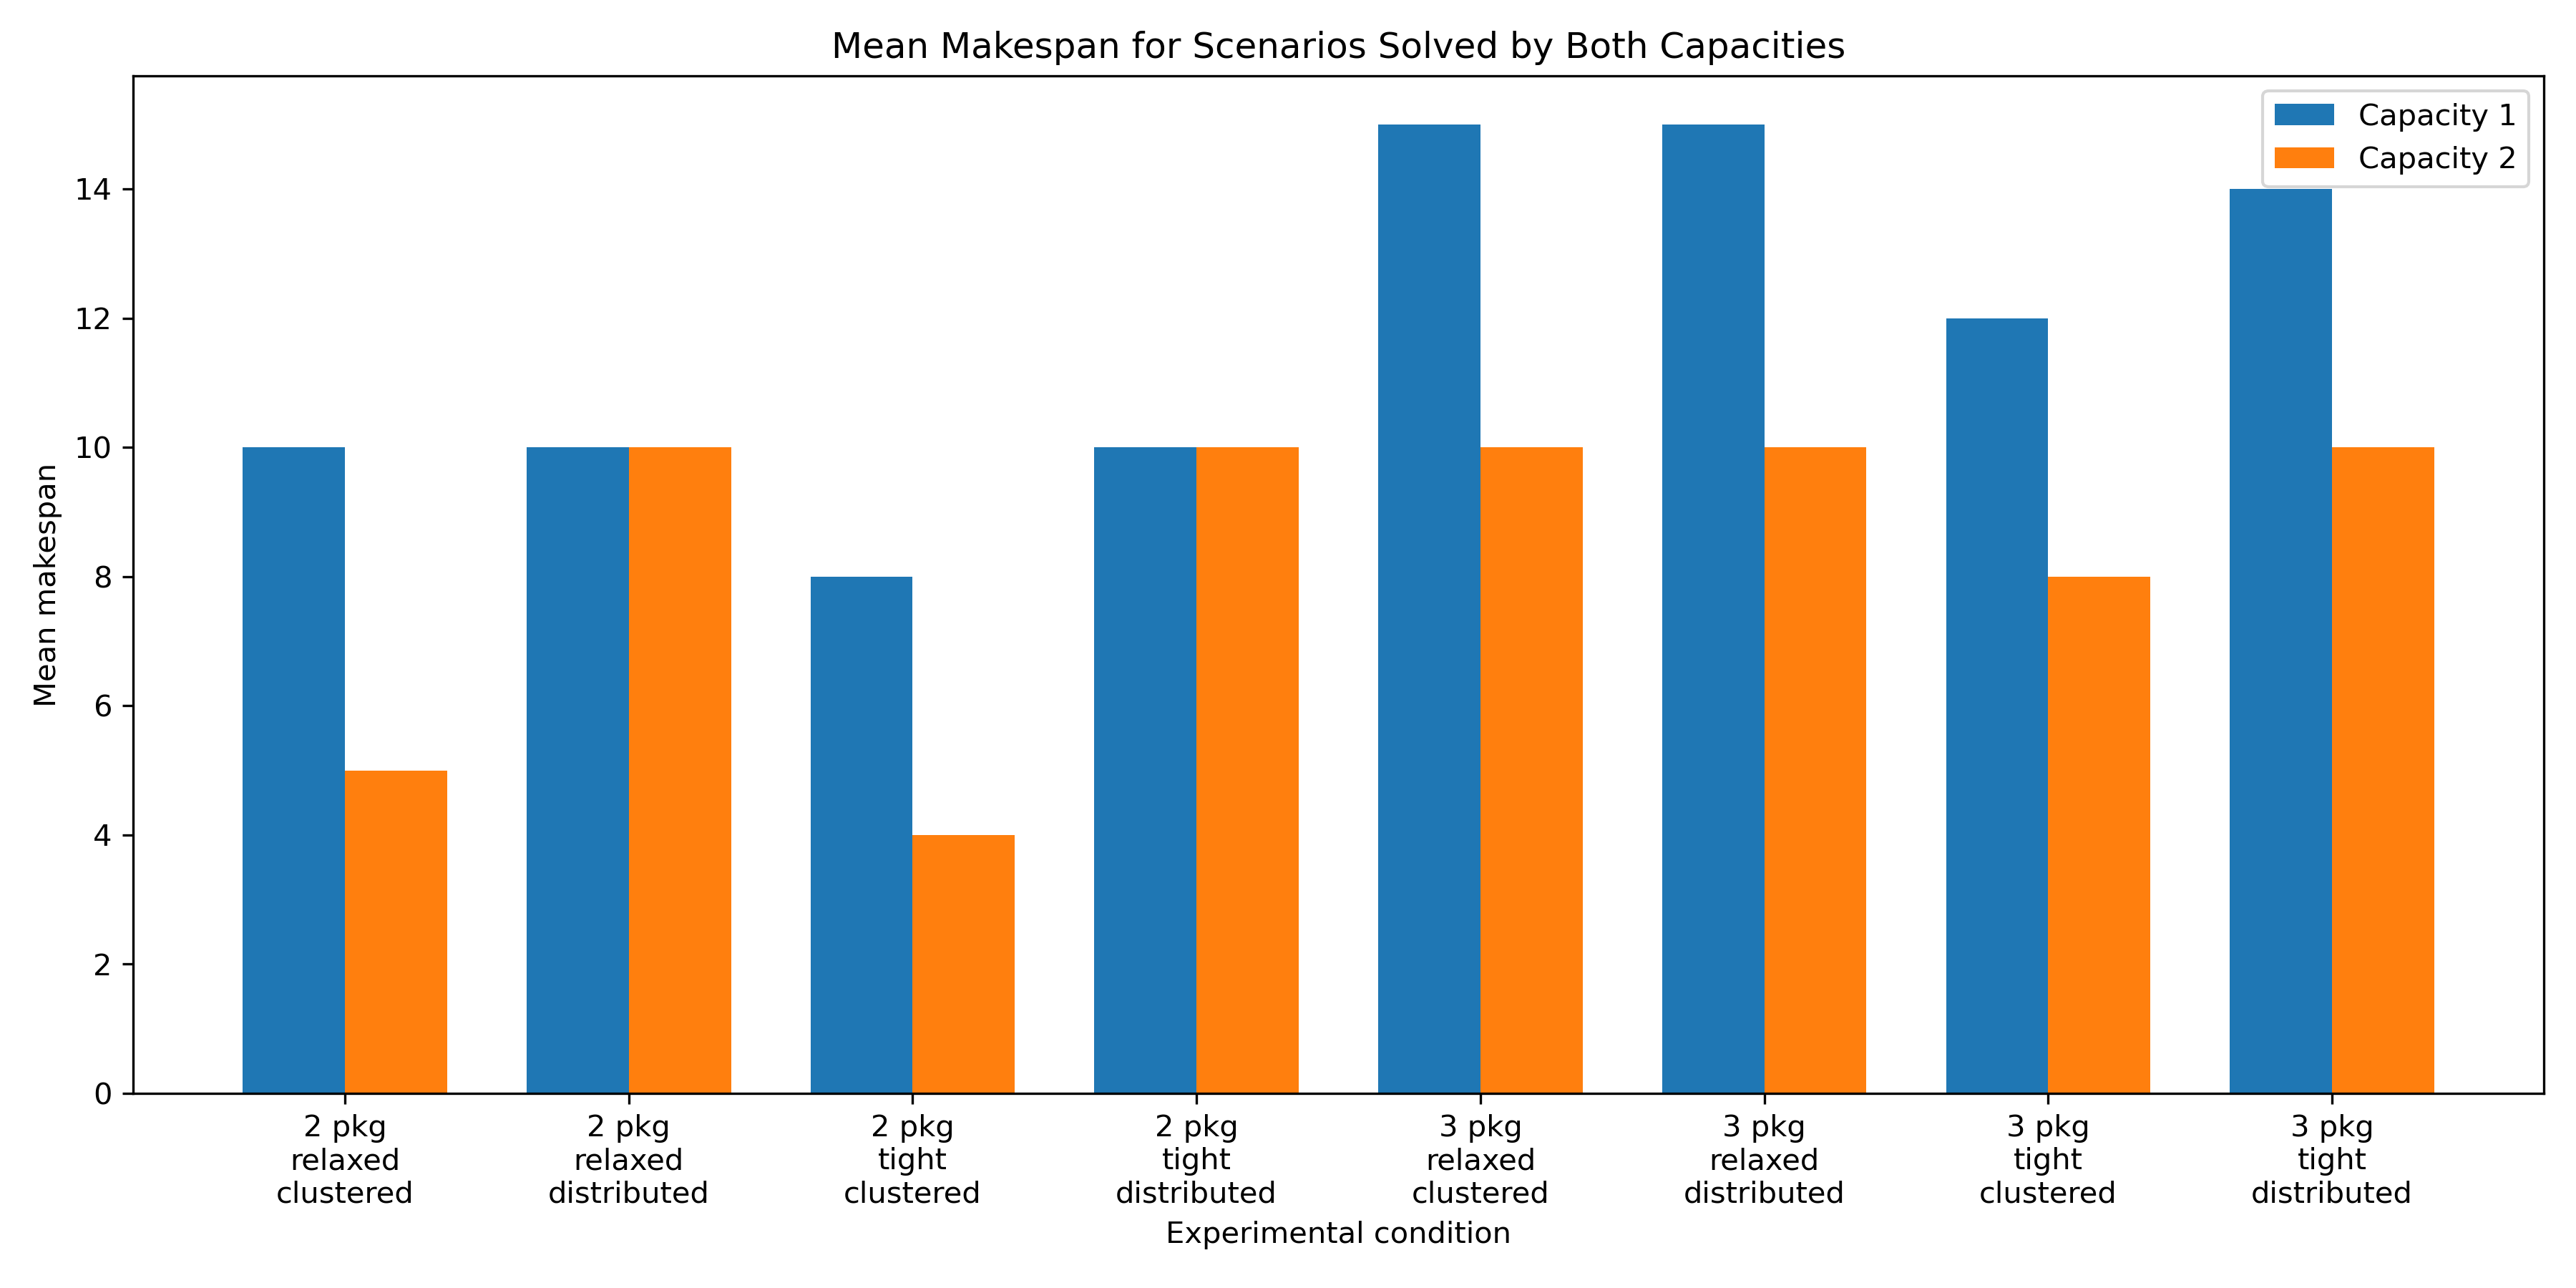
\includegraphics[width=\columnwidth]{figures/makespan_by_condition.png}
\caption{Mean makespan for scenarios solved by both capacities.}
\label{fig:makespan}
\end{figure}

For two-package distributed scenarios, mean makespan remained unchanged across
capacities. In contrast, clustered scenarios produced large reductions because
both packages could be collected during the same aisle visit.

\subsection{Search Complexity}

Capacity two also reduced planner search effort for most jointly solved
scenarios.

\begin{table}[t]
\caption{Paired Performance Results}
\centering
\begin{tabular}{lrrr}
\toprule
Metric & Cap. 1 & Cap. 2 & Reduction \\
\midrule
Makespan & 11.983 & 8.500 & 28.54\% \\
Plan length & 26.931 & 20.483 & 23.34\% \\
Expanded nodes & 12395.6 & 2544.4 & 61.93\% \\
States evaluated & 21328.6 & 5401.4 & 57.80\% \\
Planning time (ms) & 602.9 & 258.9 & 44.27\% \\
\bottomrule
\end{tabular}
\label{tab:metrics}
\end{table}

Expanded nodes decreased by 61.93\% on average
($p=2.41\times10^{-20}$), while evaluated states decreased by 57.80\%
($p=2.93\times10^{-20}$). Capacity two required less search in 108 of
116 jointly solved scenarios.

Mean planning time decreased by 44.27\% across the 114 valid runtime pairs
($p=1.75\times10^{-18}$). Because runtime is sensitive to temporary system
load, node and state counts are treated as the more robust measures of search
effort.

\begin{figure}[t]
\centering
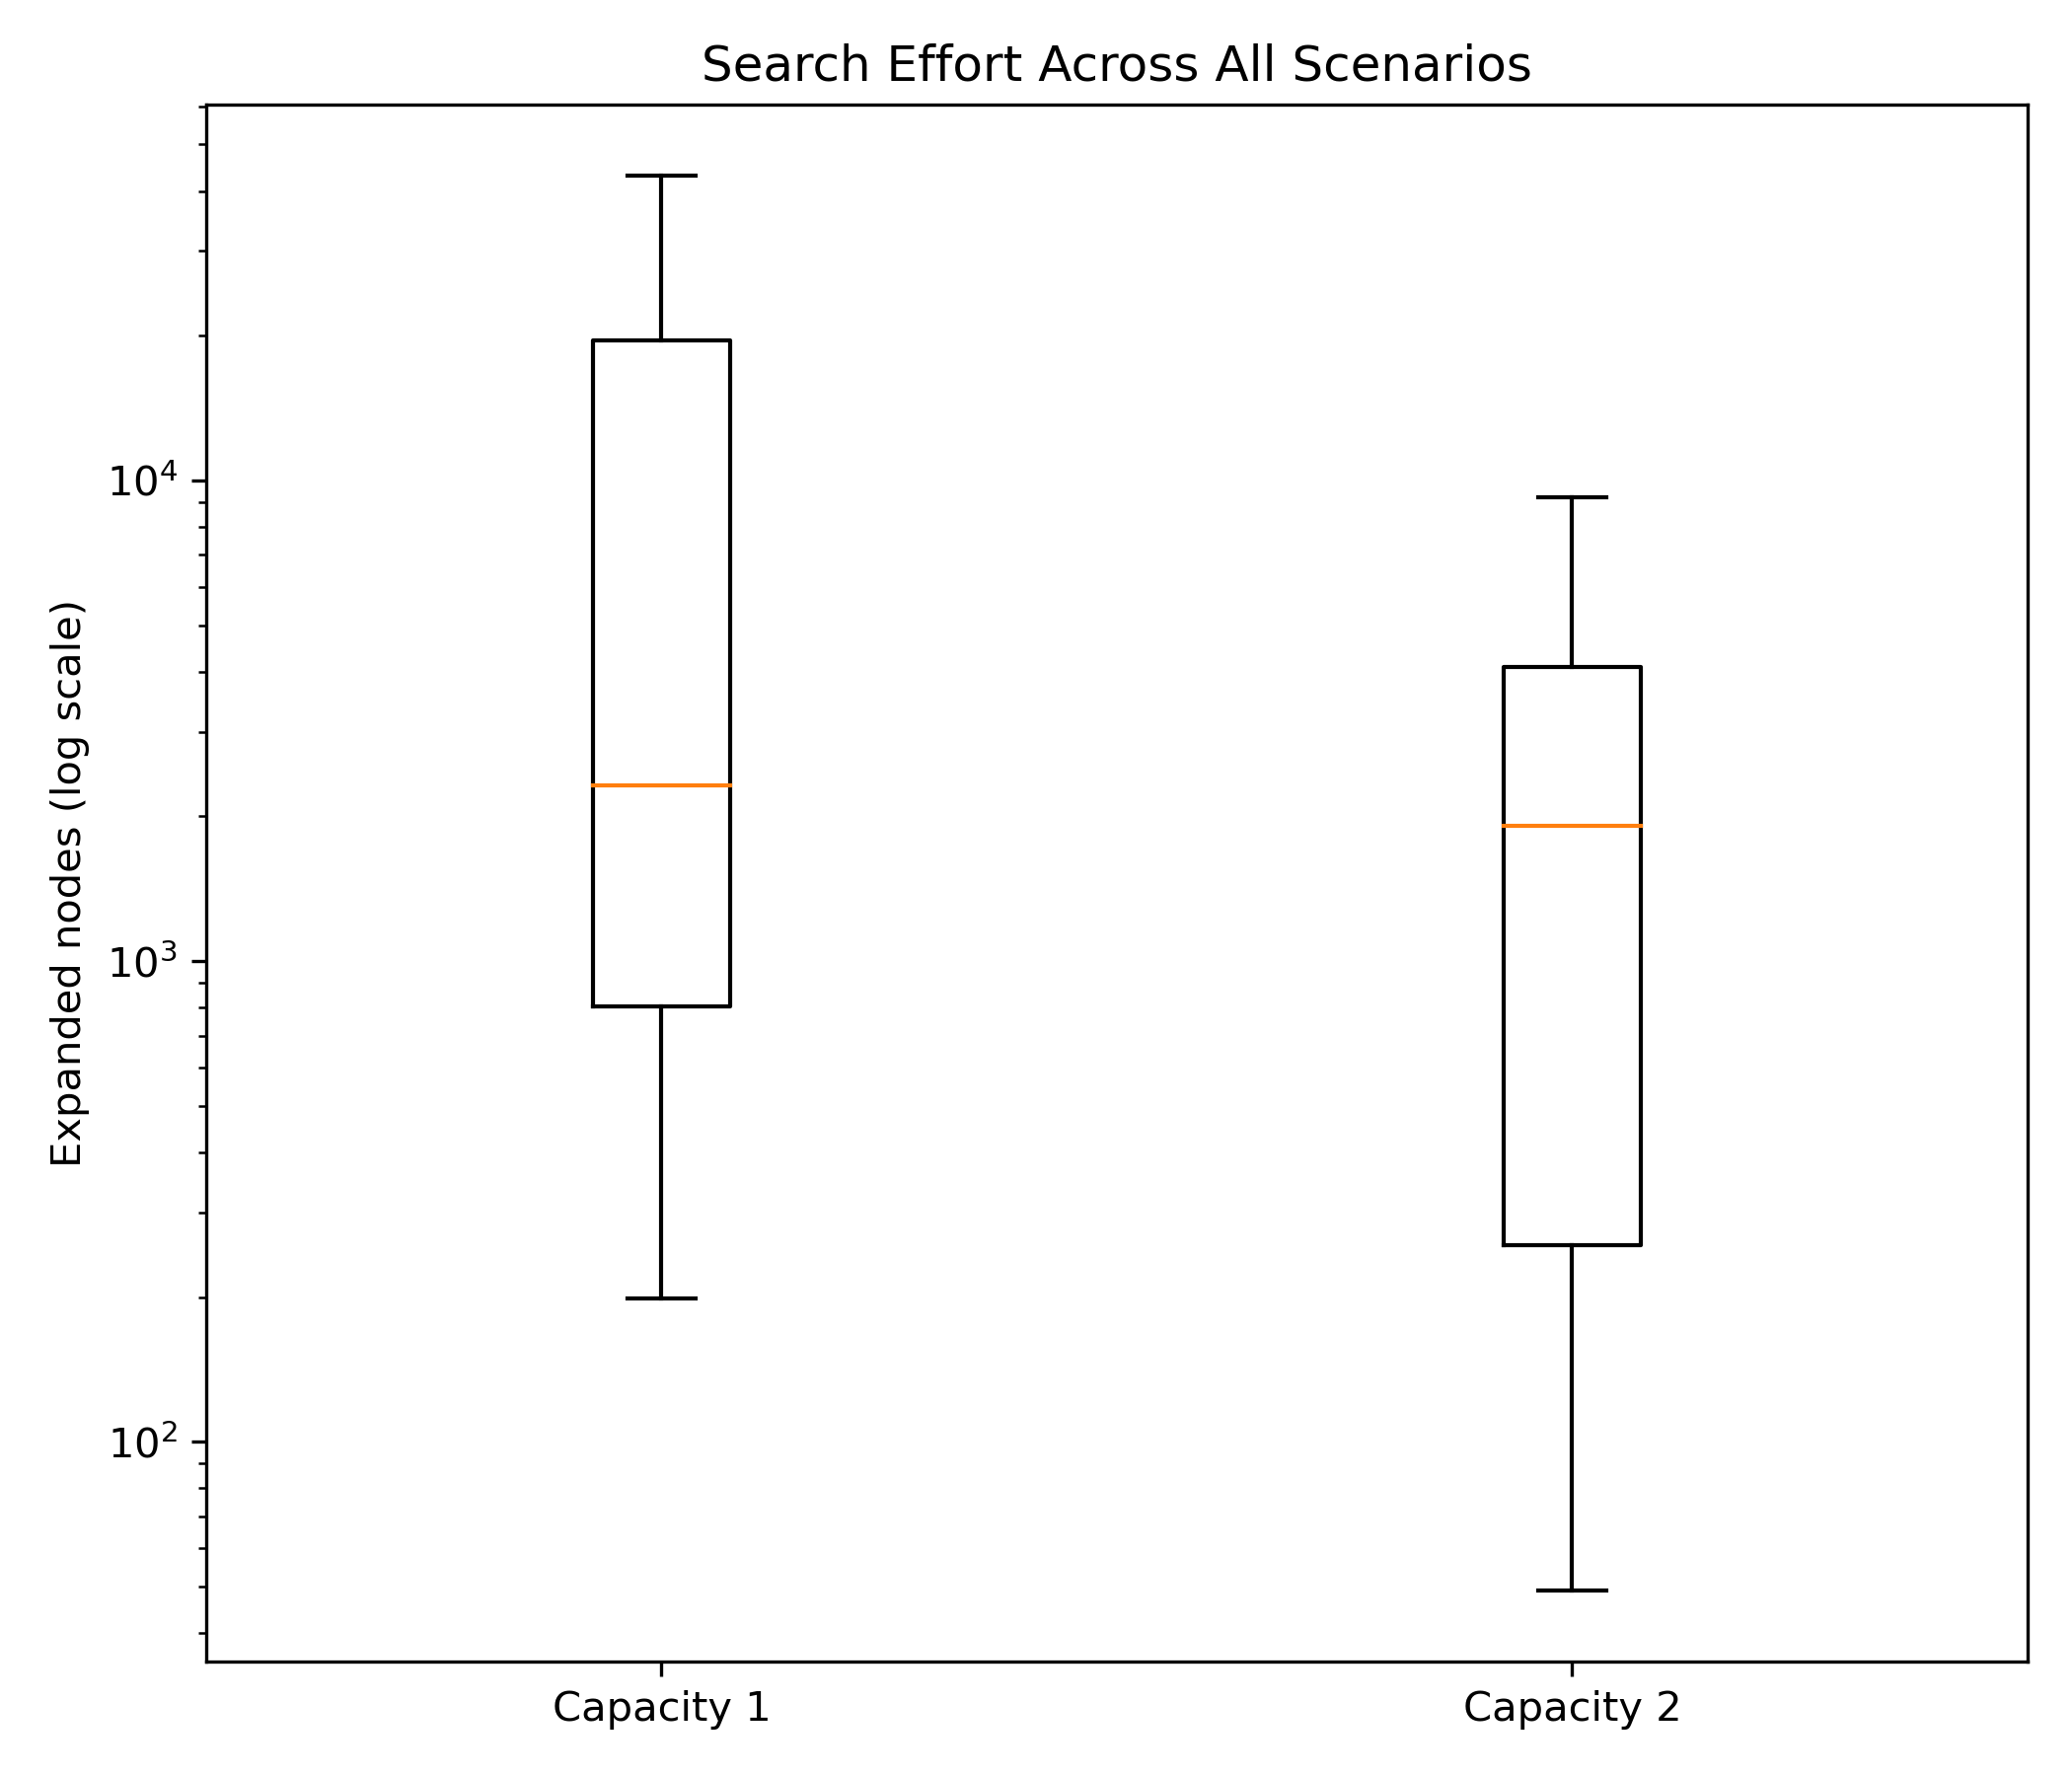
\includegraphics[width=0.85\columnwidth]{figures/expanded_nodes_boxplot.png}
\caption{Expanded-node distribution for the two capacity configurations.}
\label{fig:nodes}
\end{figure}



\subsection{ROS2 Pipeline Validation}

The batch-planning pipeline is also exposed through ROS2 and an interactive
Jupyter client. As an end-to-end consistency check, scenario 1000 was executed
under both capacities. Capacity one returned plan length 20, makespan 8,
661 expanded nodes, and 1180 evaluated states; capacity two returned plan
length 12, makespan 4, 50 expanded nodes, and 117 evaluated states. This
confirms that the Jupyter--ROS2--ENHSP interface executes the same underlying
planner workflow used by the offline experiment. The check is not counted as
an additional statistical trial.

\section{Discussion}

The results show that additional carrying capacity can influence three
different aspects of warehouse planning: feasibility, mission efficiency, and
search complexity.

The spatial interaction is particularly important. When packages are
clustered, a capacity-two robot can collect multiple packages during a single
visit, reducing repeated travel. Conversely, when two packages are placed in
different aisles, both aisles must be visited regardless of capacity. This
condition therefore provides a useful contrast showing that the improvements
cannot be attributed merely to changing a numeric model parameter.

The reduction in search effort is also notable. A larger capacity introduces
additional possible carrying states and might therefore be expected to
increase branching. In this domain, however, the planner generally reaches
shorter solution strategies and explores fewer states. Capacity two still
expanded more nodes in eight jointly solved scenarios, so the result should not
be interpreted as a general theoretical property of higher-capacity planning.



\section{Validity, Limitations, and Future Work}

\paragraph{Construct validity.}
Carrying capacity is represented directly by the numeric fluent
\texttt{max-capacity}, while \texttt{current-load} records the number of
packages carried. Solvability, makespan, plan length, expanded nodes, evaluated
states, and planning time capture complementary aspects of mission and planner
performance. However, the synthetic deadlines, symbolic package handling, and
small warehouse graph remain abstractions of an industrial system.

\paragraph{Internal and statistical validity.}
The paired design holds package locations, deadlines, geometry, package count,
layout, and random seed constant while changing only robot capacity. Separate
deterministic random streams prevent layout changes from altering deadlines.
Twenty seeds are evaluated per experimental condition. Solvability is analyzed
with an exact McNemar test and paired quantitative outcomes with the Wilcoxon
signed-rank test. Three invalid negative ENHSP timing values were treated as
missing rather than corrected or imputed.

\paragraph{External and algorithmic validity.}
The experiment uses one robot, two aisles, two or three packages, synthetic
workloads, and a single ENHSP configuration (\texttt{opt-hrmax}). The results
therefore characterize this controlled domain rather than large industrial
warehouses or all numeric planners. Four-package pilot instances showed a sharp
increase in capacity-one search effort and were excluded from the balanced
final experiment.

\paragraph{Future work.}
Future experiments should consider larger warehouse graphs, additional package
counts and capacity levels, multi-robot coordination, alternative planners and
heuristics, repeated runtime trials, and realistic warehouse order traces.

\section{Conclusion}

This work evaluated how increasing robot carrying capacity from one to two
packages affects deadline-constrained warehouse planning.

Across 160 paired scenarios, capacity two increased solvability from 72.50\%
to 93.75\%. For the 116 scenarios solved by both capacities, it reduced mean
makespan by 28.54\%, plan length by 23.34\%, expanded nodes by 61.93\%, and
evaluated states by 57.80\%.

The results also demonstrate that these benefits depend strongly on package
distribution. Additional capacity is most useful when several packages can
share part of the same route, whereas spatially separated tasks may receive
little or no route-level benefit.

Carrying capacity should therefore be considered jointly with task layout and
temporal constraints when designing warehouse planning systems.

\IEEEtriggeratref{3}
\begin{thebibliography}{13}

\bibitem{fox2006}
M. Fox and D. Long,
``Modelling Mixed Discrete-Continuous Domains for Planning,''
\emph{Journal of Artificial Intelligence Research},
vol. 27, pp. 235--297, 2006.

\bibitem{scala2016subgoal}
E. Scala, P. Haslum, and S. Thi\'ebaux,
``Heuristics for Numeric Planning via Subgoaling,''
in \emph{Proc. IJCAI}, pp. 3228--3234, 2016.

\bibitem{scala2016interval}
E. Scala, P. Haslum, S. Thi\'ebaux, and M. Ram\'irez,
``Interval-Based Relaxation for General Numeric Planning,''
in \emph{Proc. ECAI}, pp. 655--663, 2016.

\bibitem{scala2020}
E. Scala, P. Haslum, S. Thi\'ebaux, and M. Ram\'irez,
``Subgoaling Techniques for Satisficing and Optimal Numeric Planning,''
\emph{Journal of Artificial Intelligence Research},
vol. 68, pp. 691--752, 2020.

\bibitem{azadeh2019}
K. Azadeh, R. De Koster, and D. Roy,
``Robotized and Automated Warehouse Systems: Review and Recent
Developments,''
\emph{Transportation Science},
vol. 53, no. 4, pp. 917--945, 2019.

\bibitem{barros2021}
I. R. da Costa Barros and T. P. Nascimento,
``Robotic Mobile Fulfillment Systems: A Survey on Recent Developments
and Research Opportunities,''
\emph{Robotics and Autonomous Systems},
vol. 137, Art. no. 103729, 2021.

\bibitem{dumas1991}
Y. Dumas, J. Desrosiers, and F. Soumis,
``The Pickup and Delivery Problem with Time Windows,''
\emph{European Journal of Operational Research},
vol. 54, no. 1, pp. 7--22, 1991.

\bibitem{savelsbergh1995}
M. W. P. Savelsbergh and M. Sol,
``The General Pickup and Delivery Problem,''
\emph{Transportation Science},
vol. 29, no. 1, pp. 17--29, 1995.

\bibitem{fox2003}
M. Fox and D. Long,
``PDDL2.1: An Extension to PDDL for Expressing Temporal Planning Domains,''
\emph{Journal of Artificial Intelligence Research},
vol. 20, pp. 61--124, 2003.

\bibitem{coles2014}
A. J. Coles and A. Coles,
``PDDL+ Planning with Events and Linear Processes,''
in \emph{Proc. 24th International Conference on Automated Planning and
Scheduling (ICAPS)}, pp. 74--82, 2014.

\bibitem{piotrowski2016}
W. Piotrowski, M. Fox, D. Long, D. Magazzeni, and F. Mercorio,
``Heuristic Planning for PDDL+ Domains,''
in \emph{Proc. 25th International Joint Conference on Artificial
Intelligence (IJCAI)}, pp. 3213--3219, 2016.

\bibitem{wurman2008}
P. R. Wurman, R. D'Andrea, and M. Mountz,
``Coordinating Hundreds of Cooperative, Autonomous Vehicles in Warehouses,''
\emph{AI Magazine},
vol. 29, no. 1, pp. 9--19, 2008.

\bibitem{boysen2019}
N. Boysen, R. de Koster, and F. Weidinger,
``Warehousing in the E-Commerce Era: A Survey,''
\emph{European Journal of Operational Research},
vol. 277, no. 2, pp. 396--411, 2019.

\end{thebibliography}

\end{document}
